\documentclass[]{article}
\usepackage{lmodern}
\usepackage{amssymb,amsmath}
\usepackage{ifxetex,ifluatex}
\usepackage{fixltx2e} % provides \textsubscript
\ifnum 0\ifxetex 1\fi\ifluatex 1\fi=0 % if pdftex
  \usepackage[T1]{fontenc}
  \usepackage[utf8]{inputenc}
\else % if luatex or xelatex
  \ifxetex
    \usepackage{mathspec}
  \else
    \usepackage{fontspec}
  \fi
  \defaultfontfeatures{Ligatures=TeX,Scale=MatchLowercase}
\fi
% use upquote if available, for straight quotes in verbatim environments
\IfFileExists{upquote.sty}{\usepackage{upquote}}{}
% use microtype if available
\IfFileExists{microtype.sty}{%
\usepackage{microtype}
\UseMicrotypeSet[protrusion]{basicmath} % disable protrusion for tt fonts
}{}
\usepackage[margin=1in]{geometry}
\usepackage{hyperref}
\hypersetup{unicode=true,
            pdftitle={Analysis of Glucose Clamp Data},
            pdfauthor={Nathan Qi, Innocence Harvey and Dave Bridges},
            pdfborder={0 0 0},
            breaklinks=true}
\urlstyle{same}  % don't use monospace font for urls
\usepackage{longtable,booktabs}
\usepackage{graphicx,grffile}
\makeatletter
\def\maxwidth{\ifdim\Gin@nat@width>\linewidth\linewidth\else\Gin@nat@width\fi}
\def\maxheight{\ifdim\Gin@nat@height>\textheight\textheight\else\Gin@nat@height\fi}
\makeatother
% Scale images if necessary, so that they will not overflow the page
% margins by default, and it is still possible to overwrite the defaults
% using explicit options in \includegraphics[width, height, ...]{}
\setkeys{Gin}{width=\maxwidth,height=\maxheight,keepaspectratio}
\IfFileExists{parskip.sty}{%
\usepackage{parskip}
}{% else
\setlength{\parindent}{0pt}
\setlength{\parskip}{6pt plus 2pt minus 1pt}
}
\setlength{\emergencystretch}{3em}  % prevent overfull lines
\providecommand{\tightlist}{%
  \setlength{\itemsep}{0pt}\setlength{\parskip}{0pt}}
\setcounter{secnumdepth}{5}
% Redefines (sub)paragraphs to behave more like sections
\ifx\paragraph\undefined\else
\let\oldparagraph\paragraph
\renewcommand{\paragraph}[1]{\oldparagraph{#1}\mbox{}}
\fi
\ifx\subparagraph\undefined\else
\let\oldsubparagraph\subparagraph
\renewcommand{\subparagraph}[1]{\oldsubparagraph{#1}\mbox{}}
\fi

%%% Use protect on footnotes to avoid problems with footnotes in titles
\let\rmarkdownfootnote\footnote%
\def\footnote{\protect\rmarkdownfootnote}

%%% Change title format to be more compact
\usepackage{titling}

% Create subtitle command for use in maketitle
\newcommand{\subtitle}[1]{
  \posttitle{
    \begin{center}\large#1\end{center}
    }
}

\setlength{\droptitle}{-2em}
  \title{Analysis of Glucose Clamp Data}
  \pretitle{\vspace{\droptitle}\centering\huge}
  \posttitle{\par}
  \author{Nathan Qi, Innocence Harvey and Dave Bridges}
  \preauthor{\centering\large\emph}
  \postauthor{\par}
  \predate{\centering\large\emph}
  \postdate{\par}
  \date{April 7, 2017}


\begin{document}
\maketitle

{
\setcounter{tocdepth}{2}
\tableofcontents
}
\section{Data Entry}\label{data-entry}

This analysis uses the averages and errors calculated first by animal,
then averaged across groups. The clamp data is the average clamped
values.

\section{Glucose Levels During Clamp}\label{glucose-levels-during-clamp}

Glucose levels were kept the same between groups throughout the
experiment, as expected.

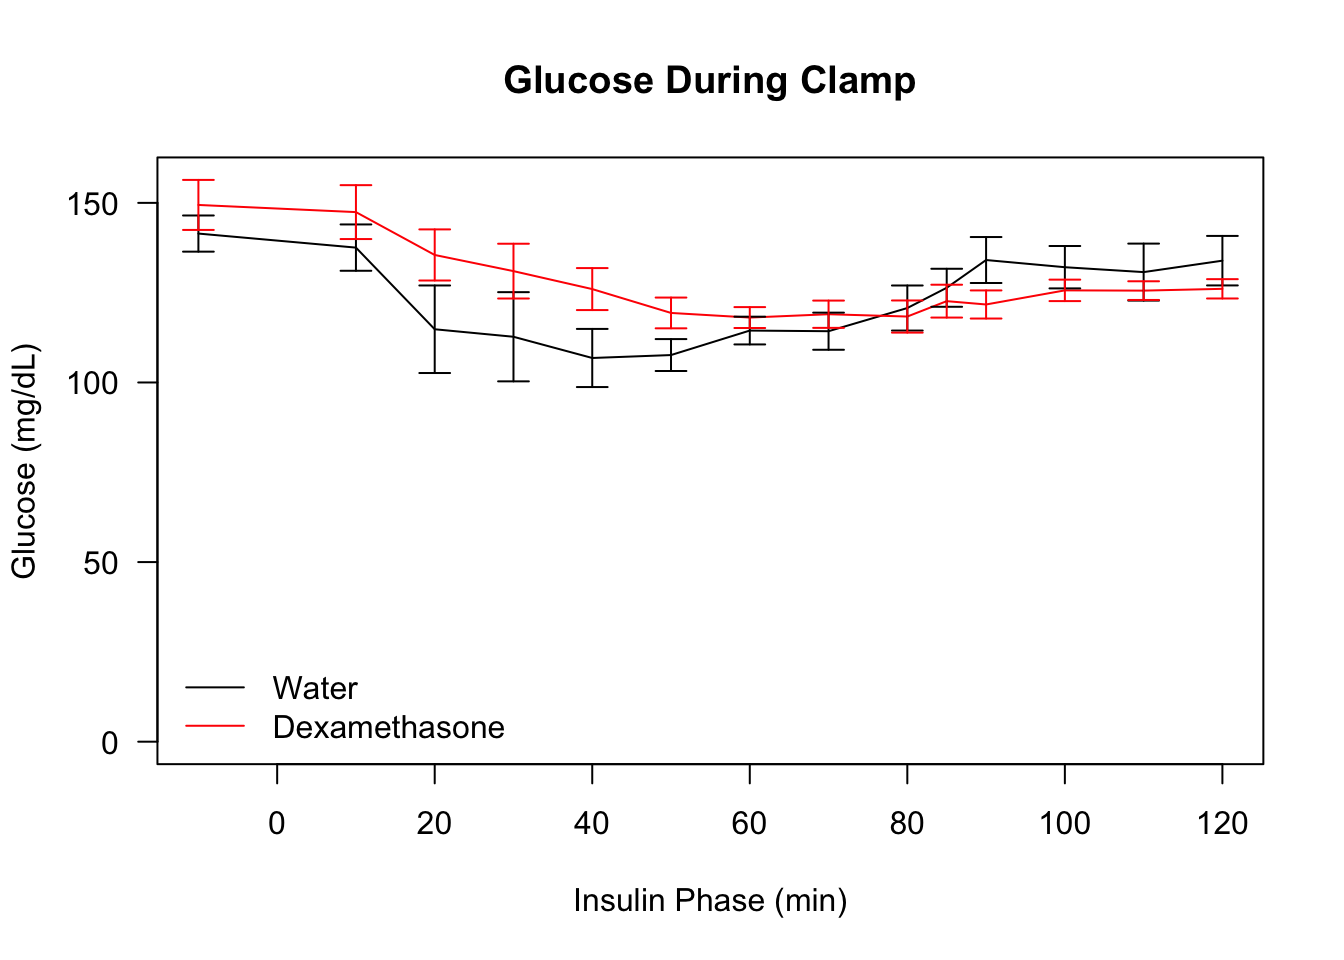
\includegraphics{figures/glucose-time-course-1.png}

During the clamp, the goal is to keep glucose constant between 120 and
130 mg/dL throughout the experiment. There was a drop in glucose levels
shortly after the insulin phase started (time 0). The following is a
linear model of Glucose levels vs time, after 80 minutes showing that
there was a significant effects of treatment on Glucose levels in this
timeframe. The dexamethasone treated group had lower blood glucose
during this phase.

\begin{longtable}[]{@{}lrrrr@{}}
\caption{Linear model of Glucose levels at the end of the clamp
phase}\tabularnewline
\toprule
term & estimate & std.error & statistic & p.value\tabularnewline
\midrule
\endfirsthead
\toprule
term & estimate & std.error & statistic & p.value\tabularnewline
\midrule
\endhead
(Intercept) & 119.697 & 5.556 & 21.55 & 0.000\tabularnewline
Time & 0.116 & 0.054 & 2.15 & 0.069\tabularnewline
TreatmentDexamethasone & -7.108 & 1.387 & -5.13 & 0.001\tabularnewline
\bottomrule
\end{longtable}

\section{Glucose Infusion Rate}\label{glucose-infusion-rate}

This only matters under insulin infusion conditions, wherein glucose
levels are decreasing due to 1) suppression of endogenous production and
2) increased clearance. As such this can be thought of as a GTT such
that if insulin requires more glucose infusion, that indicates more
insulin sensitivity. ``Glucose infusion was reduced XXX in the HFD-Dex
p=XXX.''"

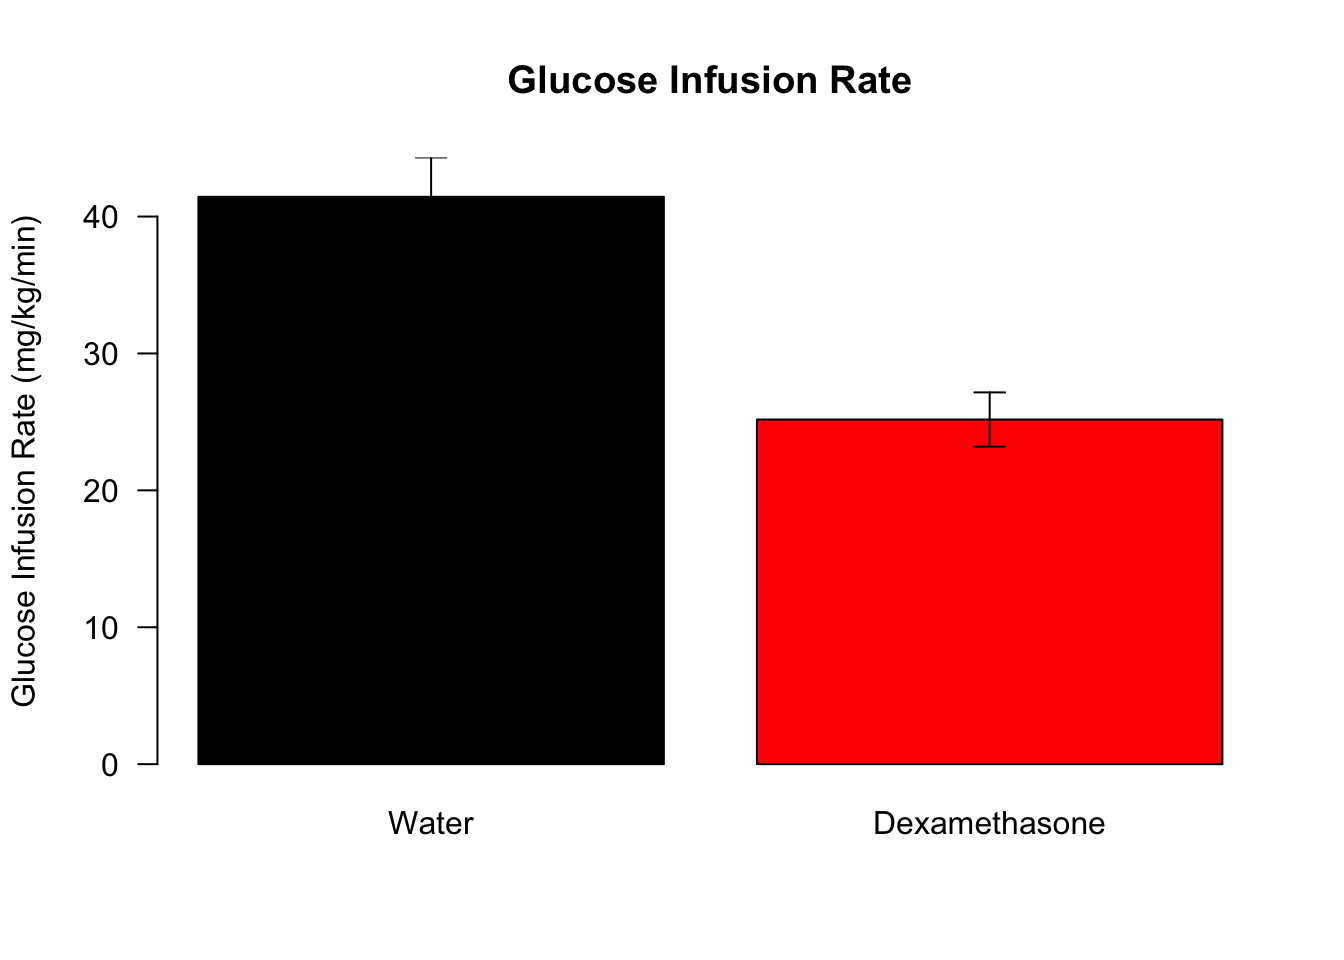
\includegraphics{figures/gir-barplot-hfd-1.png}

For the dexamethasone group, there was an average of 39.257\% reduction
in glucose infusion rates.

\begin{longtable}[]{@{}lr@{}}
\caption{Shapiro-Wilk Tests for Glucose Infusion Rates}\tabularnewline
\toprule
Treatment & Shapiro\tabularnewline
\midrule
\endfirsthead
\toprule
Treatment & Shapiro\tabularnewline
\midrule
\endhead
Water & 0.086\tabularnewline
Dexamethasone & 0.447\tabularnewline
\bottomrule
\end{longtable}

\begin{longtable}[]{@{}rrrrrrrll@{}}
\caption{Summary of t-tests for glucose infusion rates}\tabularnewline
\toprule
estimate1 & estimate2 & statistic & p.value & parameter & conf.low &
conf.high & method & alternative\tabularnewline
\midrule
\endfirsthead
\toprule
estimate1 & estimate2 & statistic & p.value & parameter & conf.low &
conf.high & method & alternative\tabularnewline
\midrule
\endhead
41.4 & 25.2 & 4.82 & 0 & 25 & 9.32 & 23.2 & Two Sample t-test &
two.sided\tabularnewline
\bottomrule
\end{longtable}

Shapiro-Wilk tests showed that the two groups could be presumed to have
equal variance, and Levene's test showed that we can assume equal
variance (p=0.736) so Student's \emph{t}-tests were used to obtain a
p-value of \textbf{0}.

This is the time course for GIR over the experiment

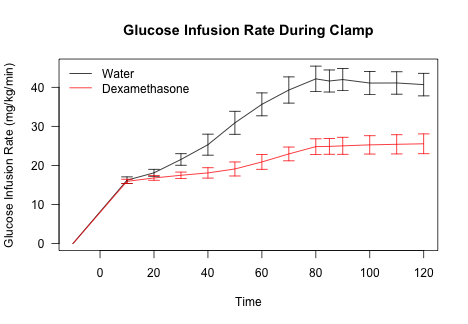
\includegraphics{figures/gir-time-course-1.png}

\section{Hepatic Glucose Production}\label{hepatic-glucose-production}

This is calculated by subtracting the Glucose turnover rates from the
glucose infusion rates:

\[ HGP = GIR - Gtr \]

Importantly at baseline (when glucose is not changing), the glucose
infusion rate is by definition zero and \(Gtr = GIR\). When insulin is
added, the glucose infusion rate increases to match glucose clearance
(to maintain euglycemia). Now all three variables have values.`Reduced
XXX in the dex but only xx in the control p=XXX'

\subsection{Glucose Production in HFD}\label{glucose-production-in-hfd}

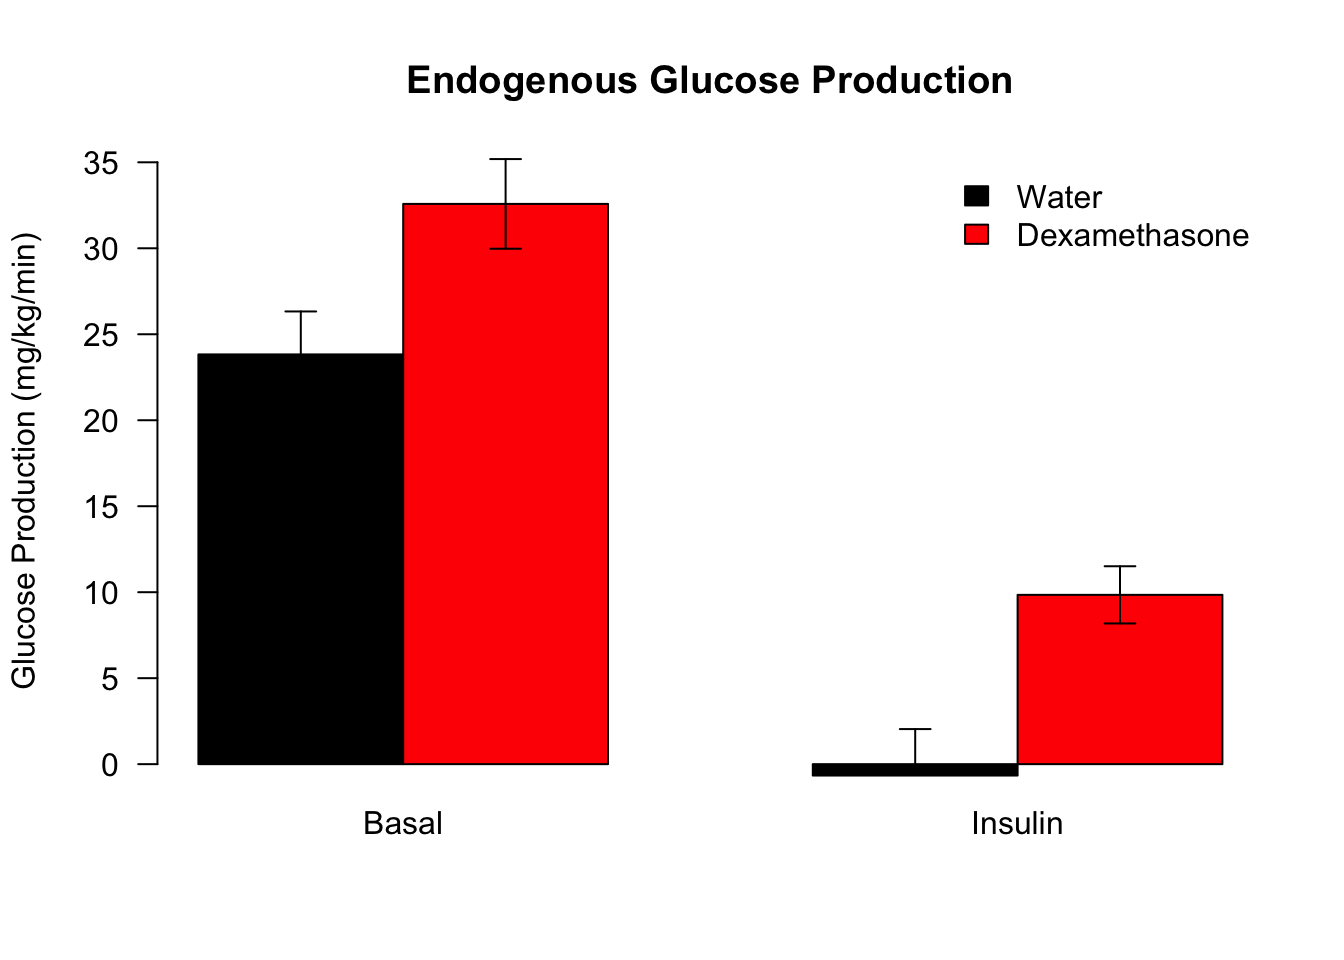
\includegraphics{figures/hgp-barplot-hfd-1.png}

Endogenous glucose production was 36.732 percent higher in the
dexamethasone-treated group in the basal condition. Under insulin
stimulated conditions, endogenous glucose production was increased from
nearly zero to 9.846 mg/kg/min (a -1588.054 fold increase). A
Shapiro-Wilk test showed that these groups were normally distributed:

\begin{longtable}[]{@{}llr@{}}
\caption{Shapiro-Wilk Tests for Basal HGP}\tabularnewline
\toprule
Treatment & Status & Shapiro\tabularnewline
\midrule
\endfirsthead
\toprule
Treatment & Status & Shapiro\tabularnewline
\midrule
\endhead
Water & Basal & 0.306\tabularnewline
Water & Insulin & 0.952\tabularnewline
Dexamethasone & Basal & 0.686\tabularnewline
Dexamethasone & Insulin & 0.323\tabularnewline
\bottomrule
\end{longtable}

\begin{longtable}[]{@{}lrrrrrrrll@{}}
\caption{Summary of t-tests for endogenous glucose
production}\tabularnewline
\toprule
& estimate1 & estimate2 & statistic & p.value & parameter & conf.low &
conf.high & method & alternative\tabularnewline
\midrule
\endfirsthead
\toprule
& estimate1 & estimate2 & statistic & p.value & parameter & conf.low &
conf.high & method & alternative\tabularnewline
\midrule
\endhead
Basal & 23.828 & 32.58 & -2.38 & 0.026 & 23 & -16.4 & -1.13 & Two Sample
t-test & two.sided\tabularnewline
Insulin & -0.662 & 9.85 & -3.50 & 0.002 & 25 & -16.7 & -4.33 & Two
Sample t-test & two.sided\tabularnewline
\bottomrule
\end{longtable}

A Levene's test showed that both Basal (p=0.441) and Insulin phase EGP
(p=0.276) can be presumed to have equal variance. Therefore a Student's
\emph{t}-test was used for both comparasons.

\subsection{Suppression of Hepatic Glucose
Output}\label{suppression-of-hepatic-glucose-output}

Percent reductions in glucose output relative to basal were calculated
for each mouse using the averaged HGP values \textgreater{}80 minutes

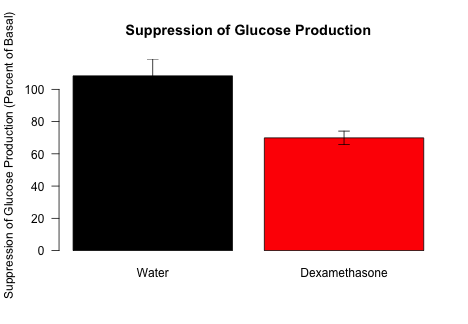
\includegraphics{figures/egp-suppression-barplot-hfd-1.png}

For the water group, there was an average of 108.369\% reduction in
glucose production, but this was only 69.905\% reduction in the
dexamethasone treated group.

\begin{longtable}[]{@{}lr@{}}
\caption{Shapiro-Wilk Tests for Suppression of HGP}\tabularnewline
\toprule
Treatment & Shapiro\tabularnewline
\midrule
\endfirsthead
\toprule
Treatment & Shapiro\tabularnewline
\midrule
\endhead
Water & 0.832\tabularnewline
Dexamethasone & 0.975\tabularnewline
\bottomrule
\end{longtable}

\begin{longtable}[]{@{}rrrrrrrll@{}}
\caption{Summary of t-tests for suppression of endogenous glucose
production}\tabularnewline
\toprule
estimate1 & estimate2 & statistic & p.value & parameter & conf.low &
conf.high & method & alternative\tabularnewline
\midrule
\endfirsthead
\toprule
estimate1 & estimate2 & statistic & p.value & parameter & conf.low &
conf.high & method & alternative\tabularnewline
\midrule
\endhead
108 & 69.9 & 3.87 & 0.001 & 25 & 18 & 58.9 & Two Sample t-test &
two.sided\tabularnewline
\bottomrule
\end{longtable}

Shapiro-Wilk tests showed that the two groups could be presumed to have
equal variance, and Levene's test showed that we can assume equal
variance (p=0.007) so Student's \emph{t}-tests were used to obtain a
p-value of \textbf{0.001}.

\section{Glucose Turnover}\label{glucose-turnover}

This is calculated by the rate of tracer infusion divided by the
specific activity of the tracer. It should increase with insulin and
represents the glucose that is taken up by the body. At the basal level
this is equal to the HGP since the GIR is zero.

Glucose turnover is significantly higher in HFD dex vs.~controls
(p=0.0262) during the basal period (not in the presence of insulin);
however, this difference goes away during the clamp.

\subsection{Glucose Turnover on HFD}\label{glucose-turnover-on-hfd}

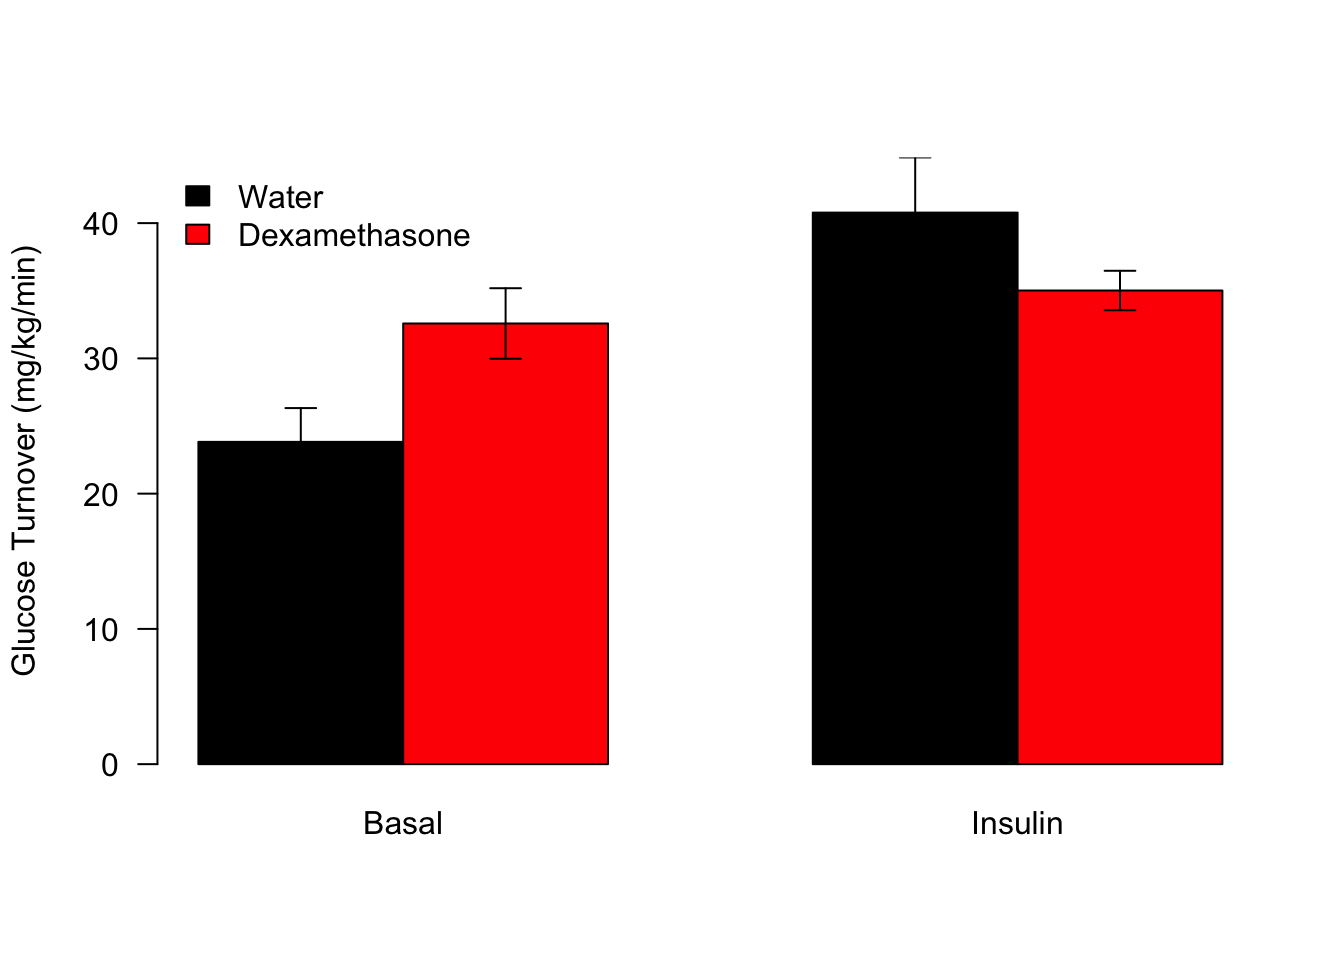
\includegraphics{figures/gtr-barplot-hfd-1.png}

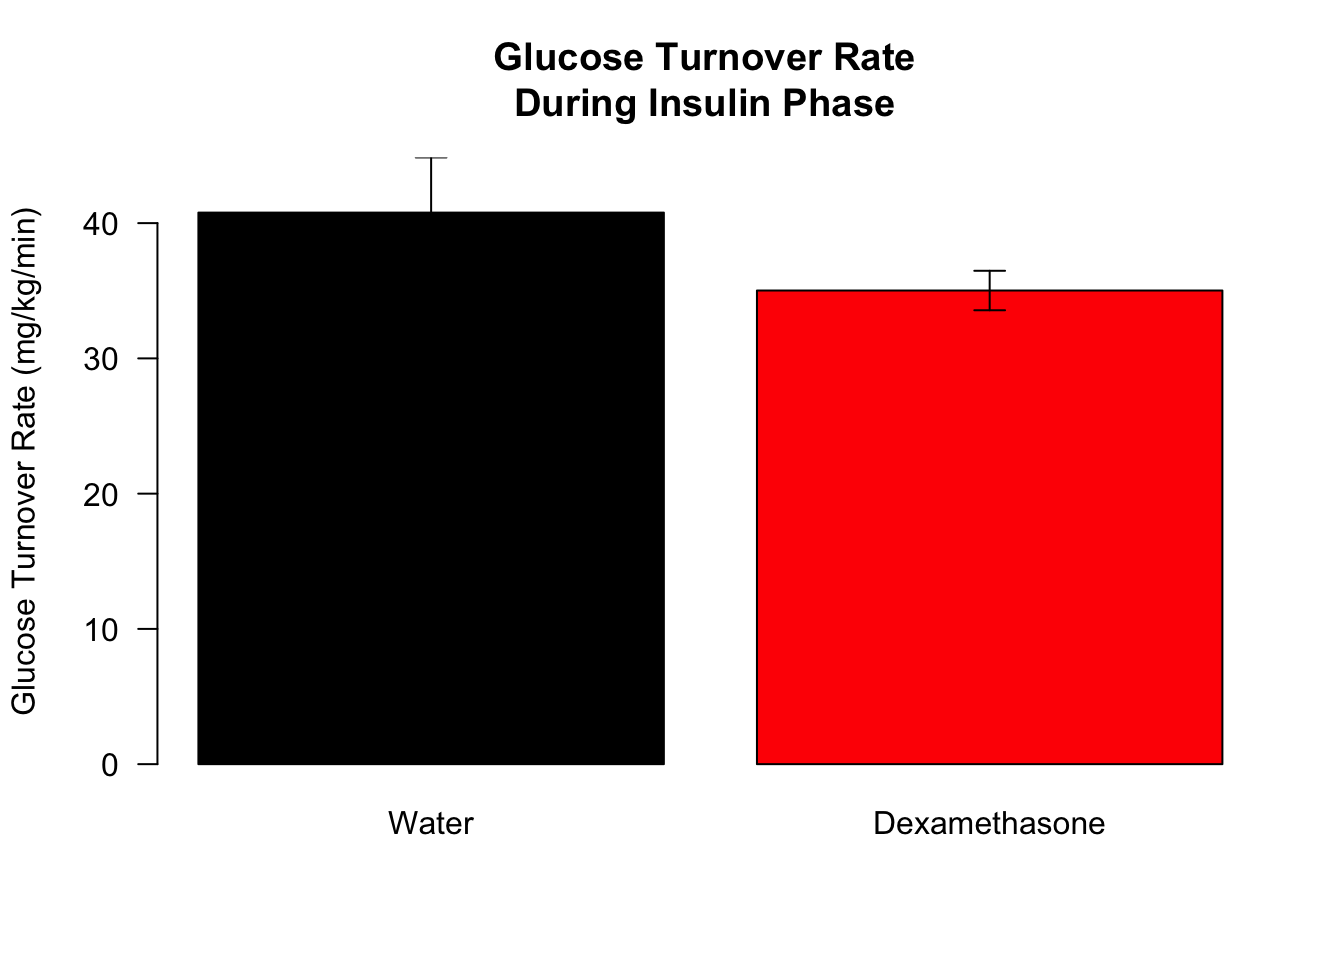
\includegraphics{figures/gtr-barplot-hfd-insulin-1.png}

For the dexamethasone group, there was a 14.126\% reduction in glucose
turnover during the insulin phase.

\begin{longtable}[]{@{}lr@{}}
\caption{Shapiro-Wilk Tests for glucose turnover during the insulin
phase}\tabularnewline
\toprule
Treatment & Shapiro\tabularnewline
\midrule
\endfirsthead
\toprule
Treatment & Shapiro\tabularnewline
\midrule
\endhead
Water & 0.536\tabularnewline
Dexamethasone & 0.501\tabularnewline
\bottomrule
\end{longtable}

\begin{longtable}[]{@{}rrrrrrrll@{}}
\caption{Summary of t-tests for glucose turnover during the insulin
phase}\tabularnewline
\toprule
estimate1 & estimate2 & statistic & p.value & parameter & conf.low &
conf.high & method & alternative\tabularnewline
\midrule
\endfirsthead
\toprule
estimate1 & estimate2 & statistic & p.value & parameter & conf.low &
conf.high & method & alternative\tabularnewline
\midrule
\endhead
40.8 & 35 & 1.52 & 0.141 & 25 & -2.05 & 13.6 & Two Sample t-test &
two.sided\tabularnewline
\bottomrule
\end{longtable}

Shapiro-Wilk tests showed that the two groups could be presumed to have
equal variance, and Levene's test showed that we can assume equal
variance (p=0.027) so Student's \emph{t}-tests were used to obtain a
p-value of \textbf{0.141}.

\section{Insulin and Glucose Levels During the
Clamp}\label{insulin-and-glucose-levels-during-the-clamp}

\subsection{Insulin levels}\label{insulin-levels}

Insulin levels were significantly higher in the basal period in the
dex-treated mice (p=0.0001) there was no difference between the groups
during the clamp.

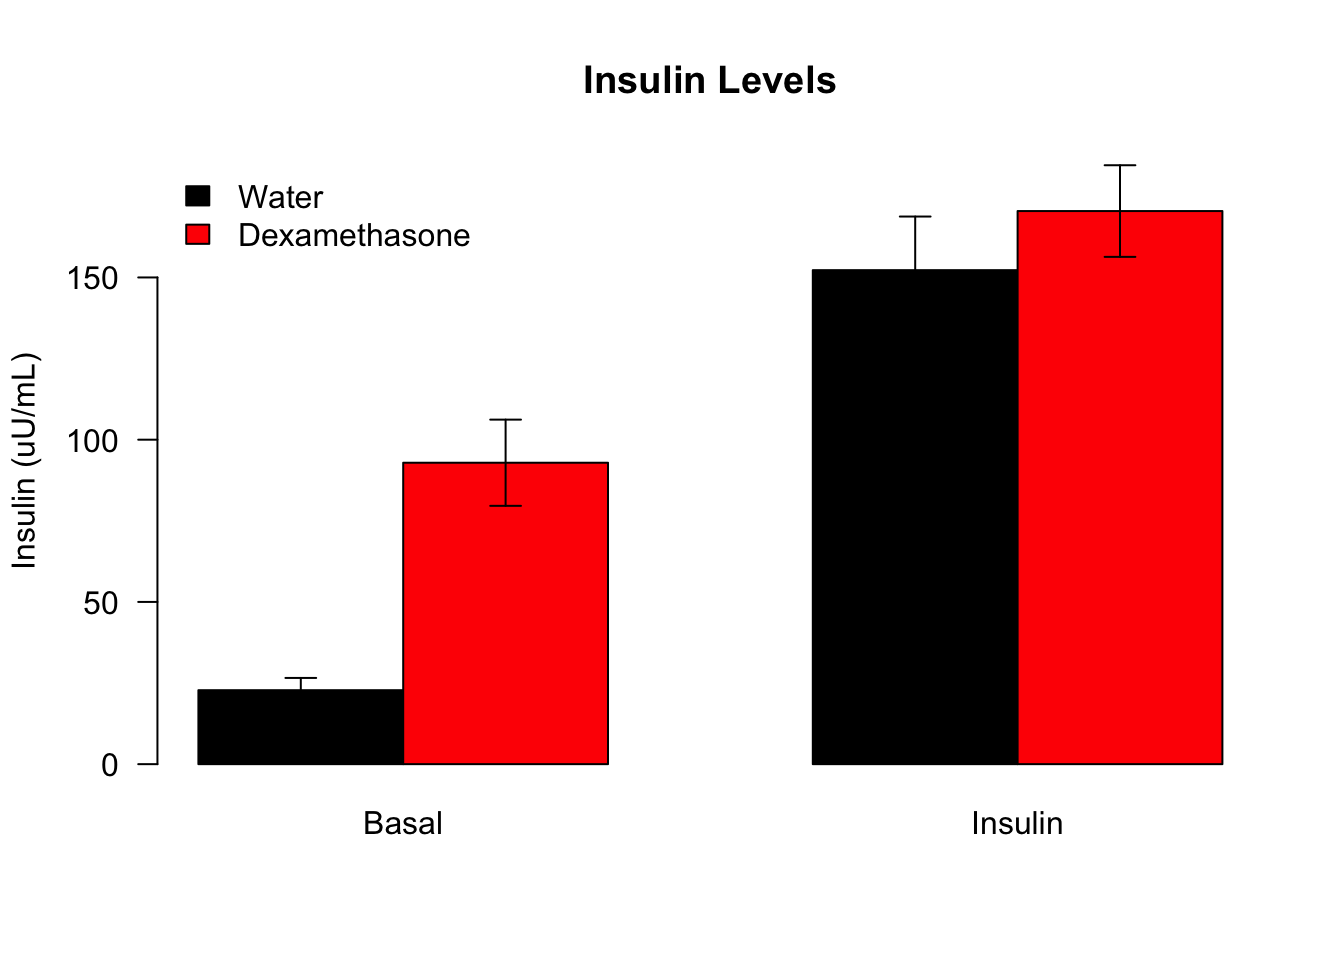
\includegraphics{figures/insulin-barplot-hfd-1.png}

\subsection{Insulin Clearance Rates}\label{insulin-clearance-rates}

There was no difference in insulin clearance between the groups

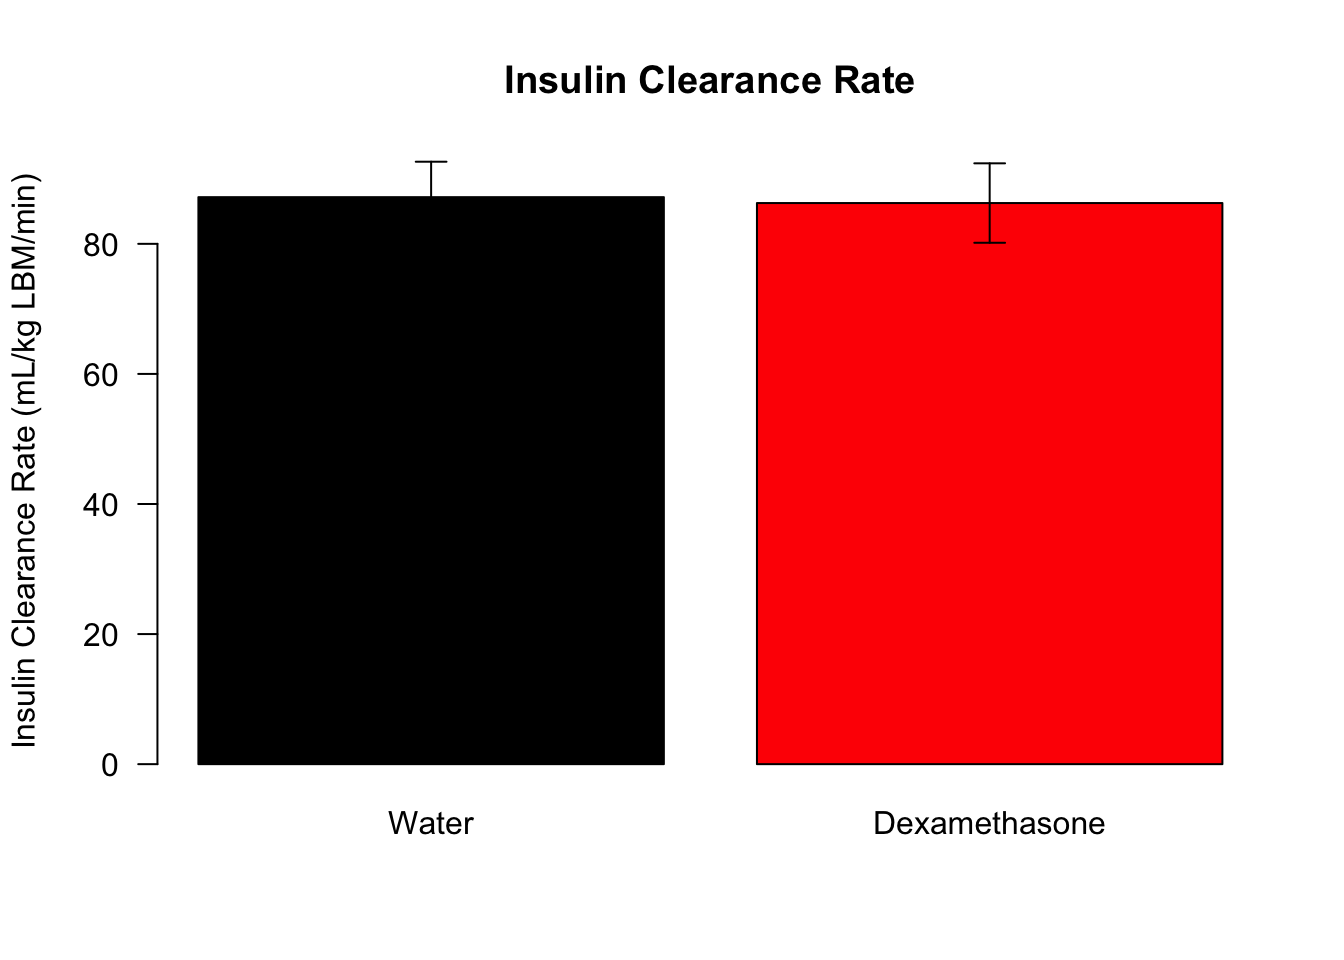
\includegraphics{figures/insulin-clearance-barplot-hfd-1.png}

For the dexamethasone group, there was only a 1.039\% reduction in
glucose infusion rates.

\begin{longtable}[]{@{}lr@{}}
\caption{Shapiro-Wilk Tests for insulin clearance rates}\tabularnewline
\toprule
Treatment & Shapiro\tabularnewline
\midrule
\endfirsthead
\toprule
Treatment & Shapiro\tabularnewline
\midrule
\endhead
Water & 0.226\tabularnewline
Dexamethasone & 0.990\tabularnewline
\bottomrule
\end{longtable}

\begin{longtable}[]{@{}rrrrrrrll@{}}
\caption{Summary of t-tests for insulin clearance rates}\tabularnewline
\toprule
estimate1 & estimate2 & statistic & p.value & parameter & conf.low &
conf.high & method & alternative\tabularnewline
\midrule
\endfirsthead
\toprule
estimate1 & estimate2 & statistic & p.value & parameter & conf.low &
conf.high & method & alternative\tabularnewline
\midrule
\endhead
87.2 & 86.3 & 0.108 & 0.915 & 23 & -16.5 & 18.3 & Two Sample t-test &
two.sided\tabularnewline
\bottomrule
\end{longtable}

Shapiro-Wilk tests showed that the two groups could be presumed to have
equal variance, and Levene's test showed that we can assume equal
variance (p=0.268) so Student's \emph{t}-tests were used to obtain a
p-value of \textbf{0.915}.

\subsection{Glucose Levels}\label{glucose-levels}

Glucose was kept similar between the groups throughout the experiment

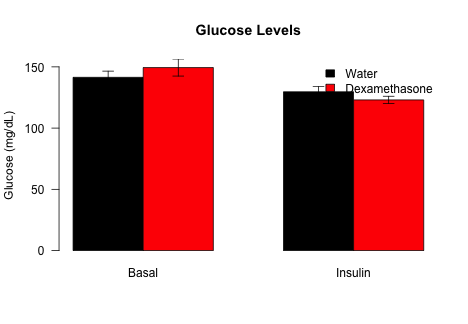
\includegraphics{figures/glucose-barplot-hfd-1.png}

\section{2-Deoxyglucose Uptake in
Tissues}\label{deoxyglucose-uptake-in-tissues}

\subsection{Inguinal Adipose Tissue}\label{inguinal-adipose-tissue}

Need to make new tables for glucose uptake data

\section{Glucose Disposal Metabolism}\label{glucose-disposal-metabolism}

\subsection{Glycolysis}\label{glycolysis}

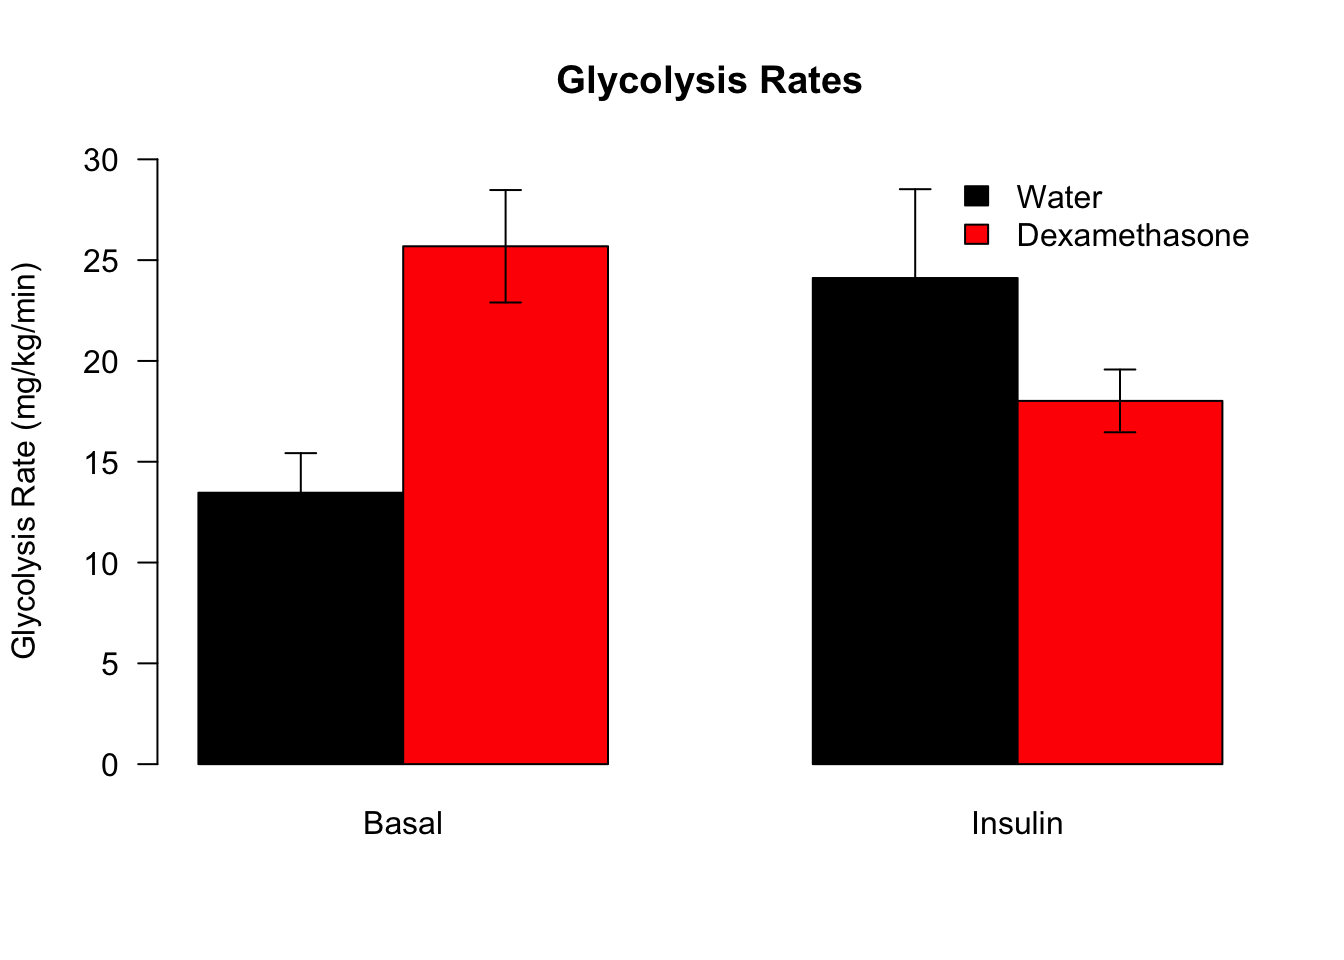
\includegraphics{figures/glycolysis-barplot-hfd-1.png}

\subsection{Glycogen Synthesis Rate}\label{glycogen-synthesis-rate}

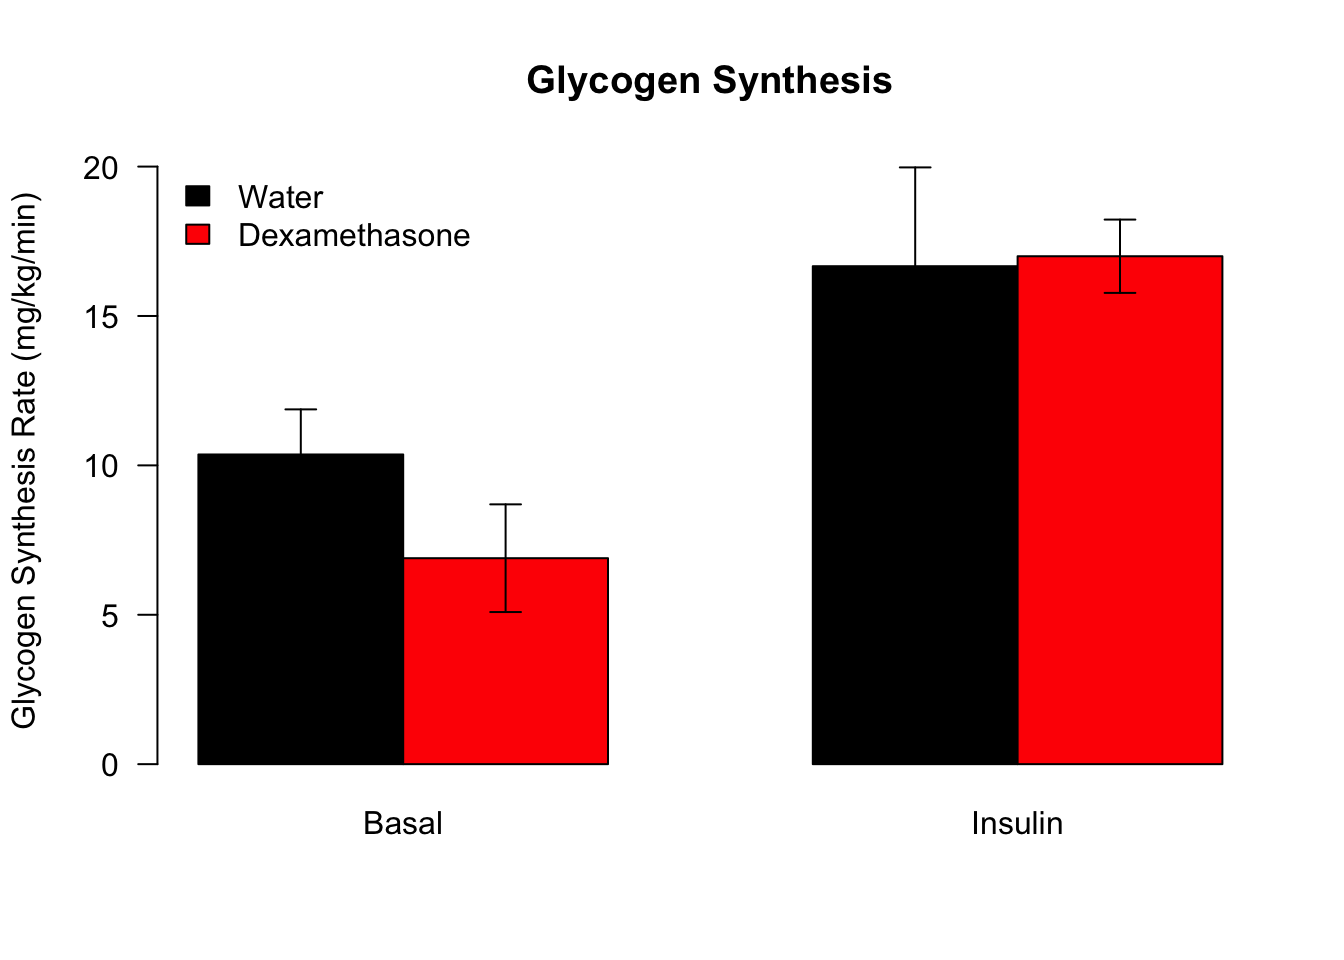
\includegraphics{figures/glycogen-barplot-hfd-1.png}

\section{Session Information}\label{session-information}

\begin{verbatim}
## R version 3.3.0 (2016-05-03)
## Platform: x86_64-apple-darwin13.4.0 (64-bit)
## Running under: OS X 10.12.6 (unknown)
## 
## locale:
## [1] en_US.UTF-8/en_US.UTF-8/en_US.UTF-8/C/en_US.UTF-8/en_US.UTF-8
## 
## attached base packages:
## [1] stats     graphics  grDevices utils     datasets  methods   base     
## 
## other attached packages:
## [1] car_2.1-4    broom_0.4.2  readr_1.1.0  dplyr_0.5.0  tidyr_0.6.1 
## [6] knitr_1.15.1
## 
## loaded via a namespace (and not attached):
##  [1] Rcpp_0.12.10       nloptr_1.0.4       plyr_1.8.4        
##  [4] highr_0.6          tools_3.3.0        digest_0.6.12     
##  [7] lme4_1.1-12        evaluate_0.10      tibble_1.3.0      
## [10] nlme_3.1-131       lattice_0.20-35    mgcv_1.8-17       
## [13] Matrix_1.2-8       psych_1.7.3.21     DBI_0.6-1         
## [16] yaml_2.1.14        parallel_3.3.0     SparseM_1.76      
## [19] stringr_1.2.0      MatrixModels_0.4-1 hms_0.3           
## [22] rprojroot_1.2      grid_3.3.0         nnet_7.3-12       
## [25] R6_2.2.0           foreign_0.8-67     rmarkdown_1.6     
## [28] minqa_1.2.4        reshape2_1.4.2     magrittr_1.5      
## [31] backports_1.0.5    htmltools_0.3.5    MASS_7.3-45       
## [34] splines_3.3.0      assertthat_0.1     pbkrtest_0.4-7    
## [37] mnormt_1.5-5       quantreg_5.29      stringi_1.1.3     
## [40] lazyeval_0.2.0
\end{verbatim}


\end{document}
